

\begin{figure}
  \begin{center}
    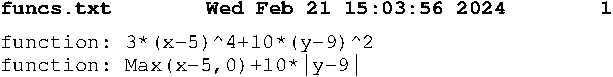
\includegraphics[width=0.95\textwidth]{funcs.pdf}
  \end{center}
  \caption{Two bivariate functions downloaded from \texttt{https://www.scss.tcd.ie/Doug.Leith/CS7DS2/week4.php}}\label{lst:funcs.txt}
\end{figure}


Let \begin{equation}
  f(x,y)=3(x-5)^4+10(y-9)^2
  \label{eq:f}
\end{equation}
and 
\begin{equation}
  g(x,y)=\max(x-5,0)+10|y-9|
  \label{eq:g}
\end{equation}

Using \texttt{sympy} we find the derivatives:
$$\nabla f=[\frac{df}{dx},\frac{df}{dy}]=[12(x-5)^{3},20y-180]$$
$$\nabla g=[\frac{dg}{dx},\frac{dg}{dy}]=[\text{Heaviside}(x-5),10\text{sign}(y-9)]$$


Clearly, the minimum of $f(x,y)$ is $0$ and they is minimized by $x=5$, $y=9$.
The other function $g(x,y)$ also has minimum $0$ but is minized by any of $x\in[-\infty,5]$ and $y=9$.


\begin{figure}
  \begin{center}
    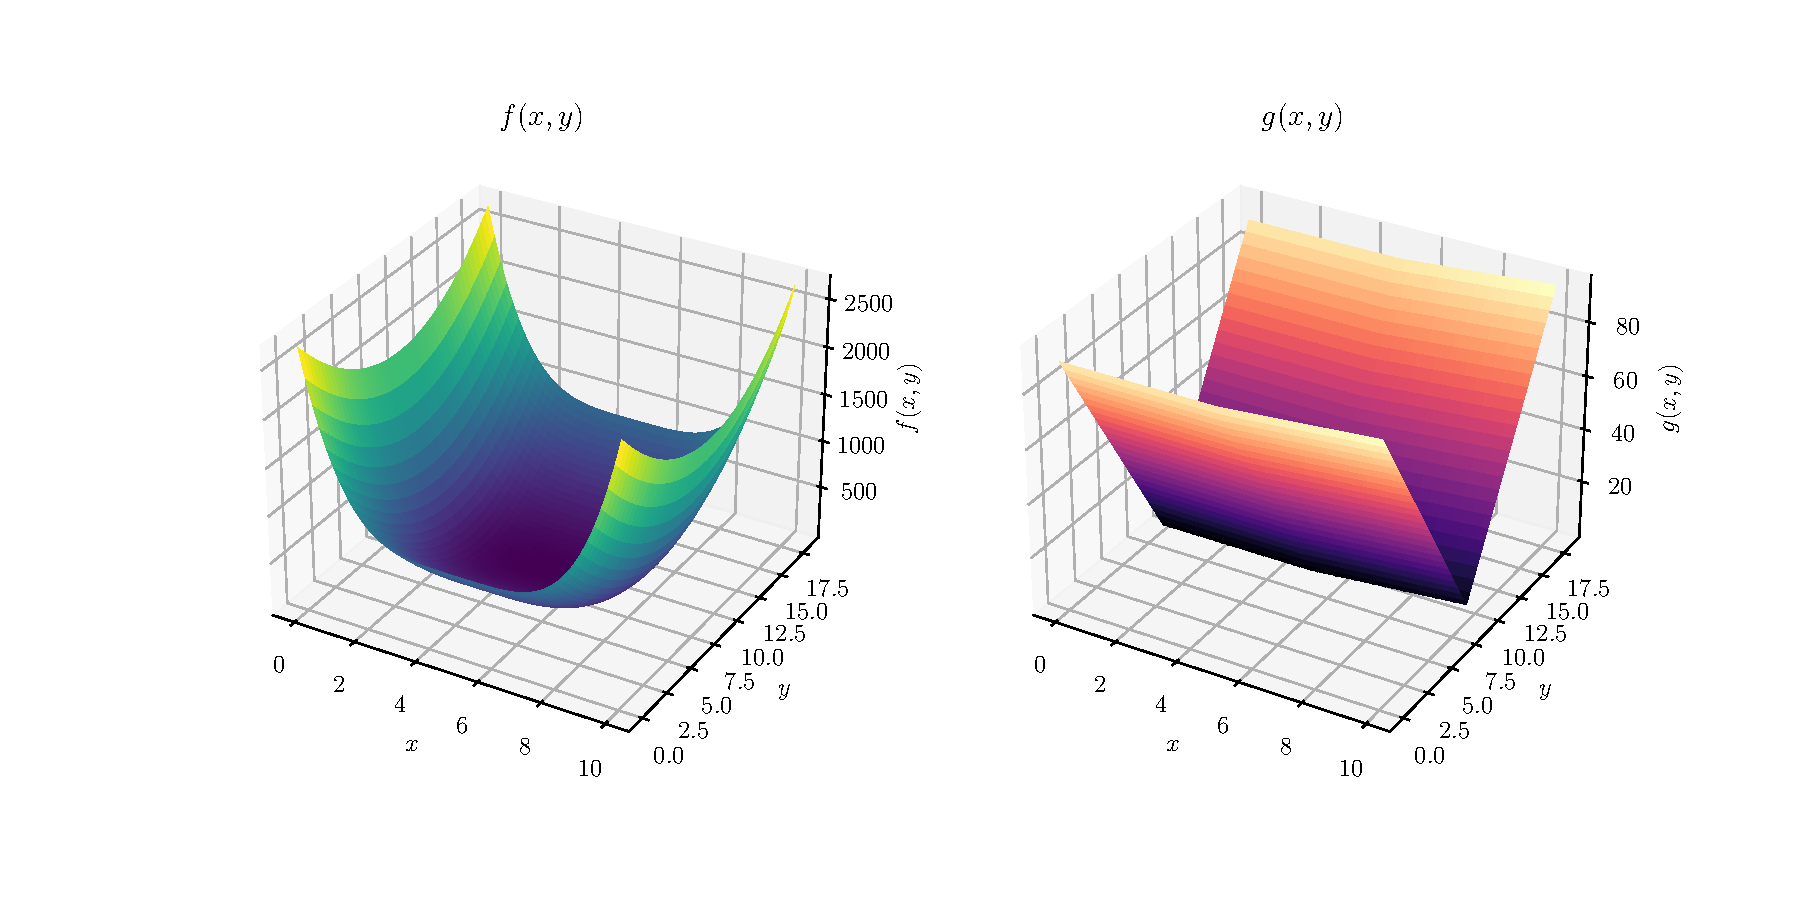
\includegraphics[width=0.95\textwidth]{fig/f-g.pdf}
  \end{center}
  \caption{}\label{fig:f-and-g}
\end{figure}

\section{(a)}
\subsection{(a) (i) Polyak}

The Polyak step size is
\begin{equation}
  \alpha_{\text{Polyak}}=\frac{f(x)-f^*}{\del f(x)^T\del f(x)}
  \label{eq:polyak-step}
\end{equation}
where $x$ is the parameter vector, $f(x)$ is the function to optimise, and $f^*\approx\min_xf(x)$.

Gradient descent iteration with Polyak step size is implemented in Listing~\ref{lst:polyak-implementation}.
The function is evaluated at the current value for $x$ and the numerator is calculated: $f(x)-f^*$.
A reasonable estimate for the minimum of the function, $f^*$, is required, here assumed to be $0$.
The dot product of the gradient is taken as the denominator. The step size is $\frac{f(x)-f^*}{\nabla f(x)^T\nabla f(x)}$.
We multiply the step size by the gradient and subtract the result from the current $x$.
\begin{listing}
  \begin{center}
    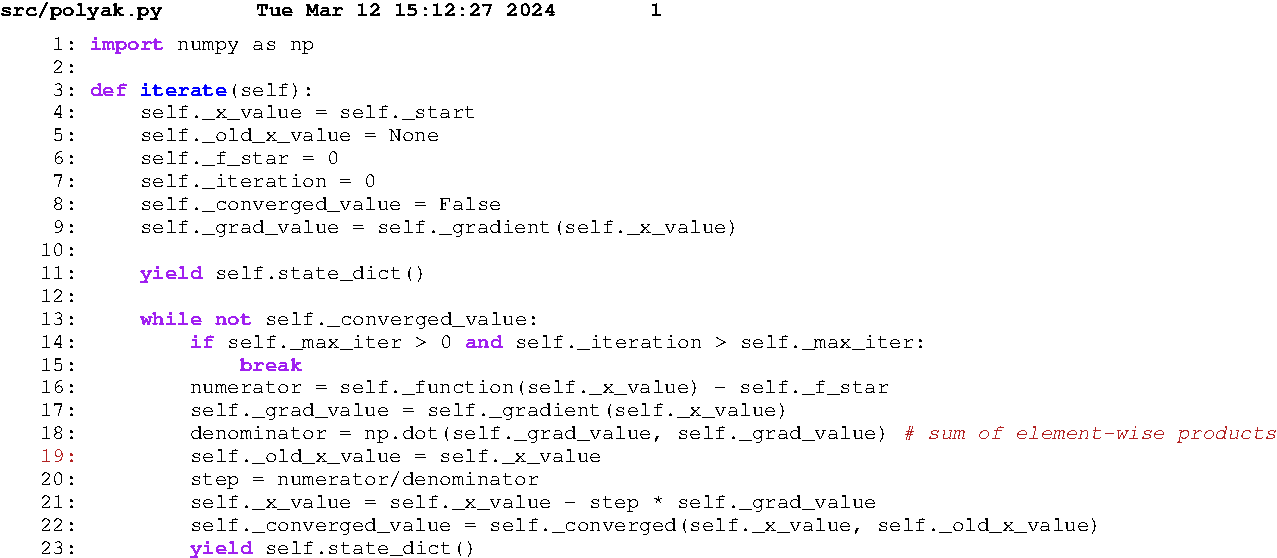
\includegraphics[width=0.95\textwidth]{fig/polyak-code.pdf}
  \end{center}
  \caption{An implementation of the update step of gradient descent using Polyak step size.}\label{lst:polyak-implementation}
\end{listing}

\subsection{(a) (ii) RMSProp}

The RMSProp step size at iteration $t$ is
\begin{equation}
  \alpha_t=\frac{\alpha_0}{\epsilon +
  \sqrt{(1-\beta)\sum_{i=0}^{t-1}\beta^{t-i}(\nabla f(x_i))^2}}
\end{equation}
and the update rule is \begin{equation}
  x_{t+1}:=x_t-\alpha_t*\nabla f(x_t)
  \label{eq:rmsprop}
\end{equation}
where $\epsilon$ is some small value to prevent divide by zero, $\alpha_0$
and $\beta$ are hyperparameters to be set, noting that $0<\beta\le1$. The
result is that previous gradients influence the current step size, but are
gradually forgotten due to the $\beta^{t-i}$ term.

A Python implementation of the update step is provided in
Listing~\ref{lst:rmsprop-implementation}. The term inside the square root
can be calculated iteratively, as in line 25 of
Listing~\ref{lst:rmsprop-implementation}.


\begin{listing}
  \begin{center}
    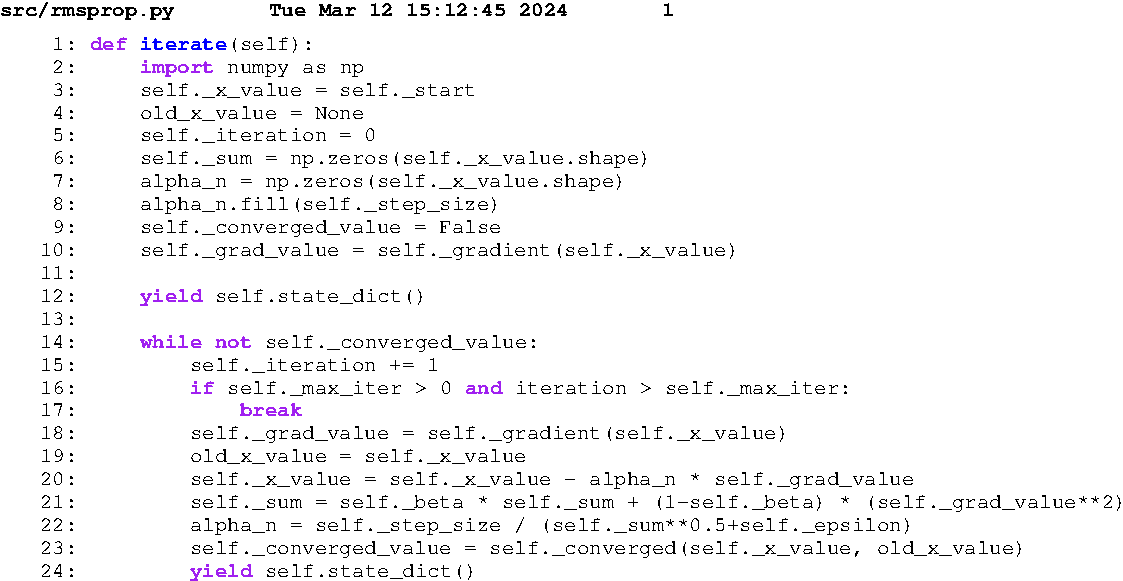
\includegraphics[width=0.95\textwidth]{fig/rmsprop-code.pdf}
  \end{center}
  \caption{An implementation of the update step of gradient descent using RMSProp step size.}\label{lst:rmsprop-implementation}
\end{listing}

\subsection{(a) (iii) Heavy Ball}

The Heavy Ball step is
\begin{equation}
  z_{t+1}=\beta z_t + \alpha\nabla f(x_t)
\end{equation}
with the update rule \begin{equation}
  x_{t+1}=x_t-z_{t+1}
\end{equation}
where t is the current iteration (starting at 0), $z_0=0$, and
$x_0$, $\alpha$, and $\beta$ have to be set.

A Python implementation of the update step is provided in Listing~\ref{lst:heavy_ball-implementation}.

\begin{listing}
  \begin{center}
    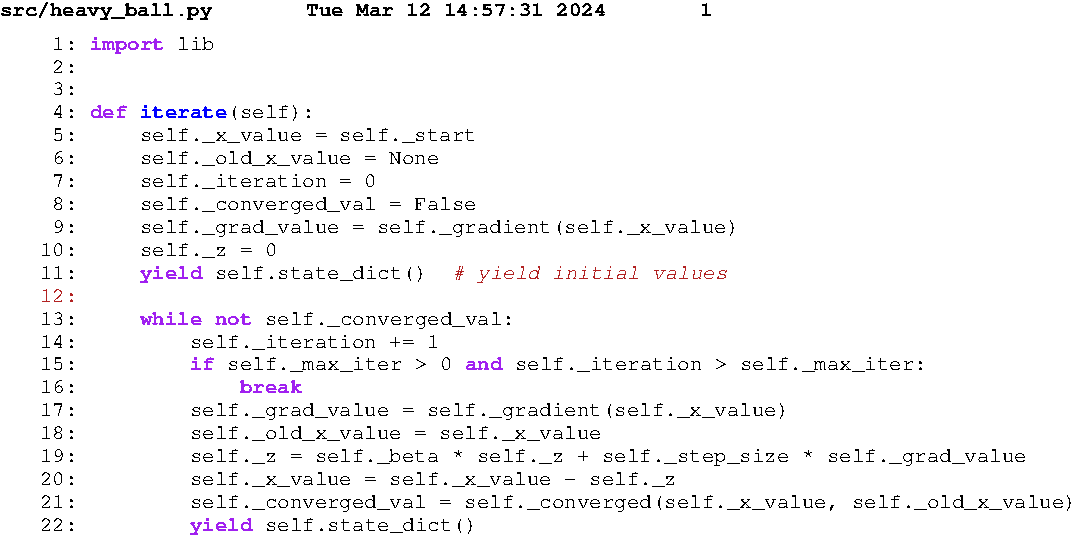
\includegraphics[width=0.95\textwidth]{fig/heavy_ball-code.pdf}
  \end{center}
  \caption{An implementation of the update step of gradient descent using Heavy Ball step size.}\label{lst:heavy_ball-implementation}
\end{listing}

\subsection{(a) (iv) Adam}

The Adam step size is calculated in terms of
\begin{equation}
  m_{t+1}=\beta_1m_t+(1-\beta_1)\nabla f(x_t)
\end{equation}
and \begin{equation}
  v_{t+1}=\beta_2v_t+(1-\beta_2)[\nabla f(x_t) \circ \nabla f(x_t)]
\end{equation}
from which we get
\begin{equation}
  \hat m=\frac{m_{t+1}}{(1-\beta_1^t)}
\end{equation}
and
\begin{equation}
  \hat v=\frac{v_{t+1}}{(1-\beta_2^t)}
\end{equation}
which are used in the update step as
\begin{equation}
  x_{t+1}=x_t-\alpha[\frac{\hat m_1}{\epsilon + \sqrt{\hat v_1}},\ldots,\frac{\hat m_n}{\epsilon + \sqrt{\hat v_n}}]
\end{equation}
where $t$ is the iteration, $\alpha$, $\beta_1$, and $\beta_2$ are hyperparameters, and $\epsilon$ is some small value to prevent divide-by-zero. The element-wise product is denoted with $\circ$.


A Python implementation of the update step is provided in Listing~\ref{lst:adam-implementation}.

\begin{listing}
  \begin{center}
    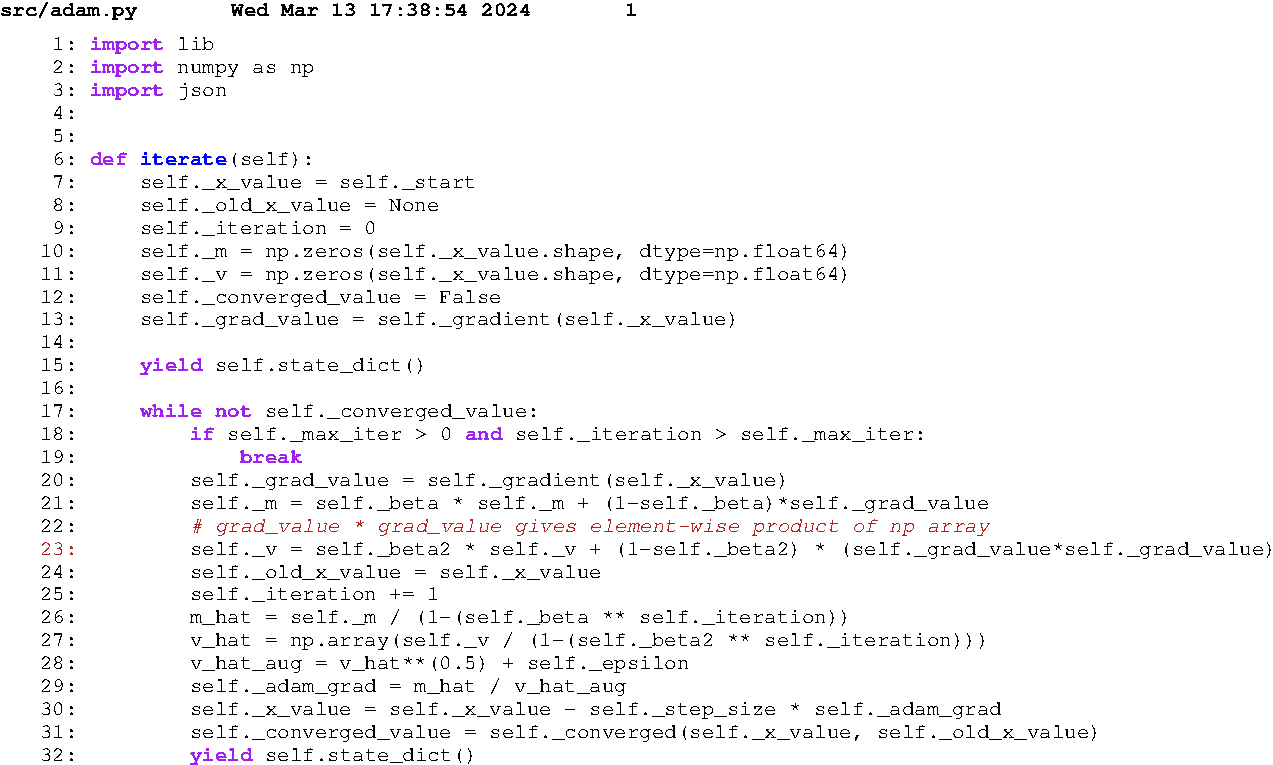
\includegraphics[width=0.95\textwidth]{fig/adam-code.pdf}
  \end{center}
  \caption{An implementation of the update step of gradient descent using Adam step size.}\label{lst:adam-implementation}
\end{listing}

\section{(b)}
In this section we look at the influence of the hyperparameters on
the behaviour gradient descent for each of RMSProp, Heavy Ball (HB), and Adam, on the functions
$f(x,y)$ and $g(x,y)$.
In each case the starting point is $(x,y)=(6,8)$.
The convergence condition is when the maximum change goes
below 0.001; $max(|x_n-x_{n+1}|,|y_n-y{n+1}|)<0.001$.

A feature of the $g(x,y)$ function is that its derivative w.r.t. $x$ is $0$ for
all $x\le5$, which means that for starting values with $x<5$, the gradient descent updates
only move in one direction. These cases are not discussed further here.

\subsection{(b) (i) RMSProp hyperparameters}
The RMSProp step size has two hyperparameters, $\alpha$, and $\beta$ (ignoring $\epsilon$ for this discussion).
The $\alpha$ parameter is the unadjusted step size, and the $\beta$ parameter controls
how quickly previous gradients decay in the calculation of subsequent step sizes.
A lower $\beta$ means faster decay, so in the limit as $\beta$ goes to $0$,
RMSProp approaches the constant step size algorithm.
As we increase $\beta$ we assign more weight to the gradients from older iterations
in terms of the next step size.

Various runs of gradient descent with RMSProp are presented
in Figure~\ref{fig:rms-step-plots}, with function $f$ on the
left and $g$ on the right. The top two plots show the
progression of $f(x,y)$ and $g(x,y)$ respectively through
iterations. We find that with $\beta=0.25$ we can push
$\alpha$ up to 0.4 without diverging, but with $\beta=0.9$
we diverge, for $f$. Similarly for $g$ the lower $\beta=0.25$
allows us to push $\alpha$ up to 0.5 without diverging, whereas
the higher $\beta=0.9$ causes divergence.

An interesting behaviour of the RMSProp step size is that
it can suddenly explode when the gradient is very
small on successive iterations.
This is caused by the denominator of $\alpha_t$
becoming very small.
This means that when the estimate gets very close to
the true minimum (and hence the gradient is very small for $f$)
the step size can explode, causing the algorithm to
start exploring again.

\begin{figure}
  \begin{center}
    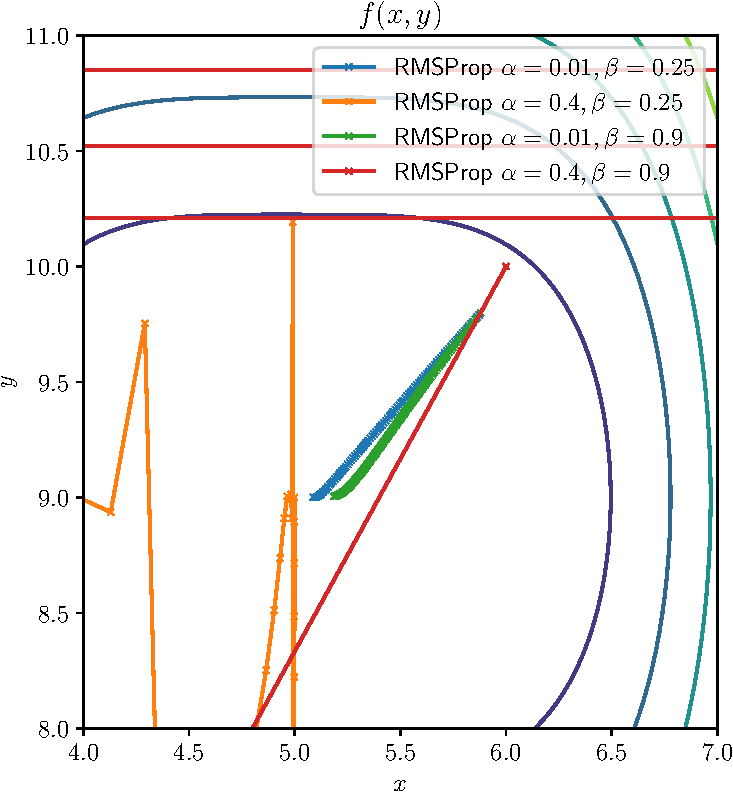
\includegraphics[width=0.45\textwidth]{fig/rmsprop-step-plot-f.pdf}
    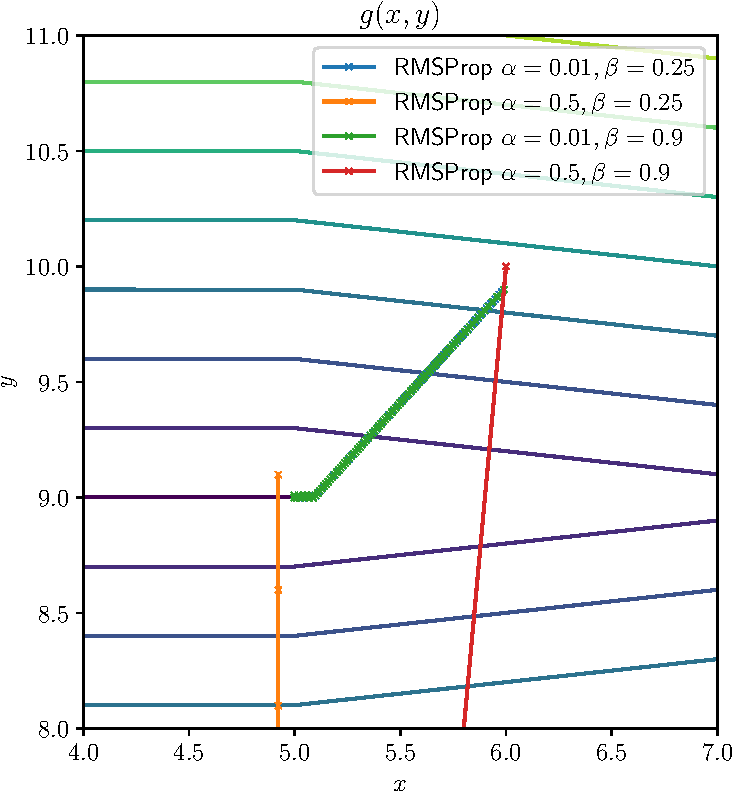
\includegraphics[width=0.45\textwidth]{fig/rmsprop-step-plot-g.pdf}

    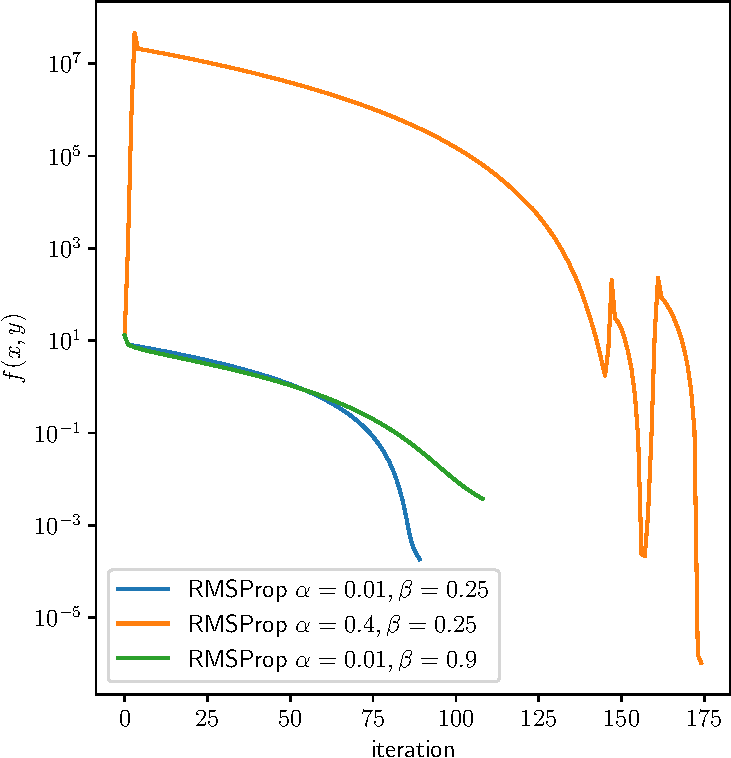
\includegraphics[width=0.45\textwidth]{fig/rmsprop-iterations-f.pdf}
    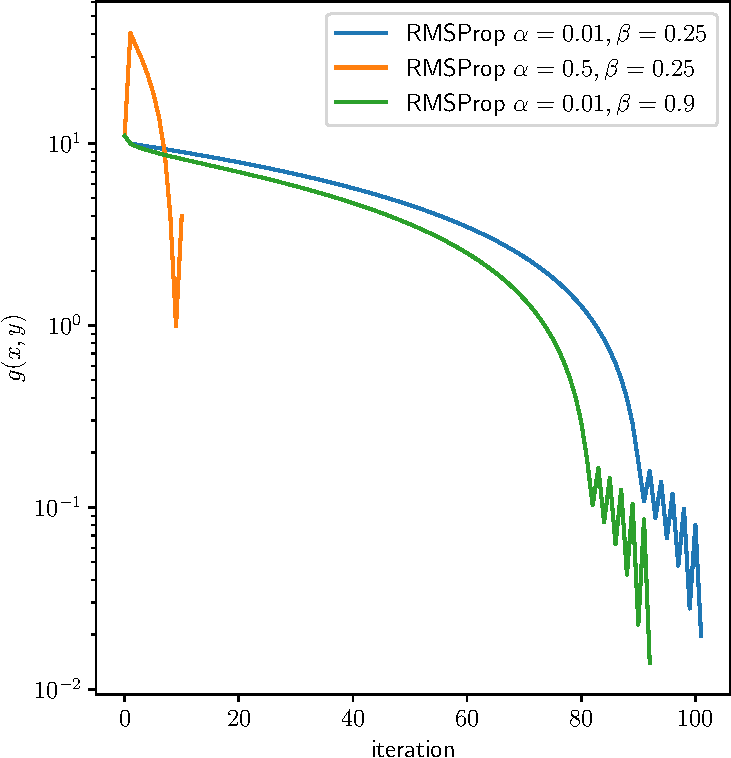
\includegraphics[width=0.45\textwidth]{fig/rmsprop-iterations-g.pdf}
  \end{center}
  \caption{Various runs of gradient descent with different RMSProp hypers.}\label{fig:rms-step-plots}
\end{figure}

\subsection{(b) (ii) Heavy Ball hyperparameters}
Heavy Ball also has two hyperparameters, $\alpha$ and $\beta$, but
does include the normalization term $\frac{1}{(1-\beta)}$, as in RMSProp.
As the number of iterations increases the step can be factored
to approximately $(1+\beta+\beta^2+...)=1/(1-\beta)$, which means
we are effectively scaling the baseline $\alpha$ parameter:
$\alpha/(1-\beta)$, which means a larger $\beta$ results
in larger steps, once we have warmed up with some
iterations. In the top left plot of Figure~\ref{fig:heavy_ball-step-plots} we see that the steps stay larger for longer
when $\beta=0.9$ compared to $\beta=0.25$.

Looking at the green line in the top right plot of Figure~\ref{fig:heavy_ball-step-plots} we see that the
movement starts of going left, but after $x$ is less than
5 the gradient in the $x$ axis is 0 and so the
momentum gradually decreases.

\begin{figure}
  \begin{center}
    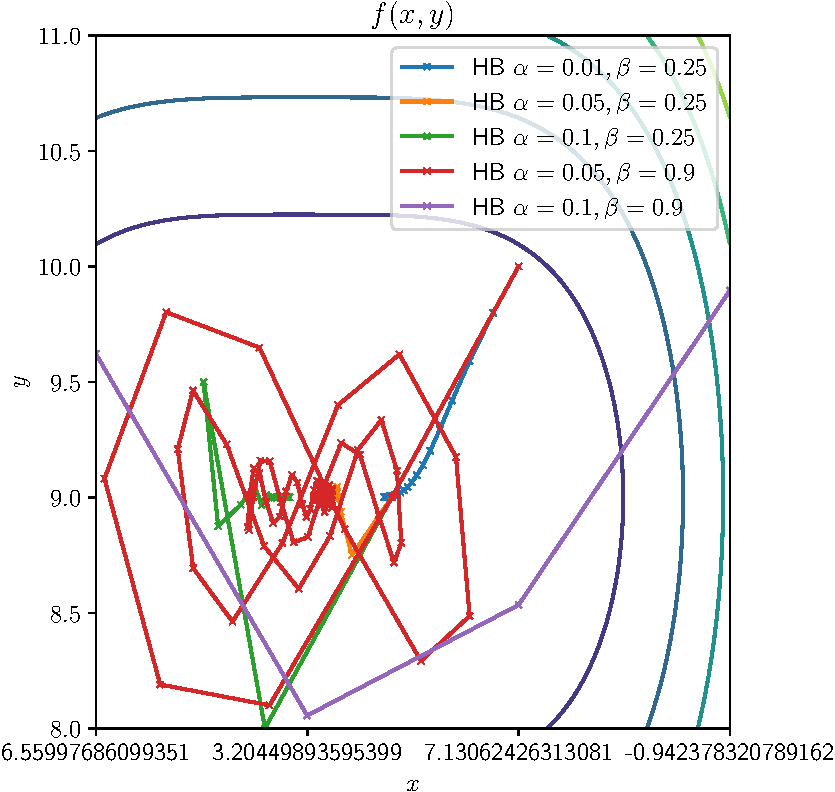
\includegraphics[width=0.45\textwidth]{fig/heavy_ball-step-plot-f.pdf}
    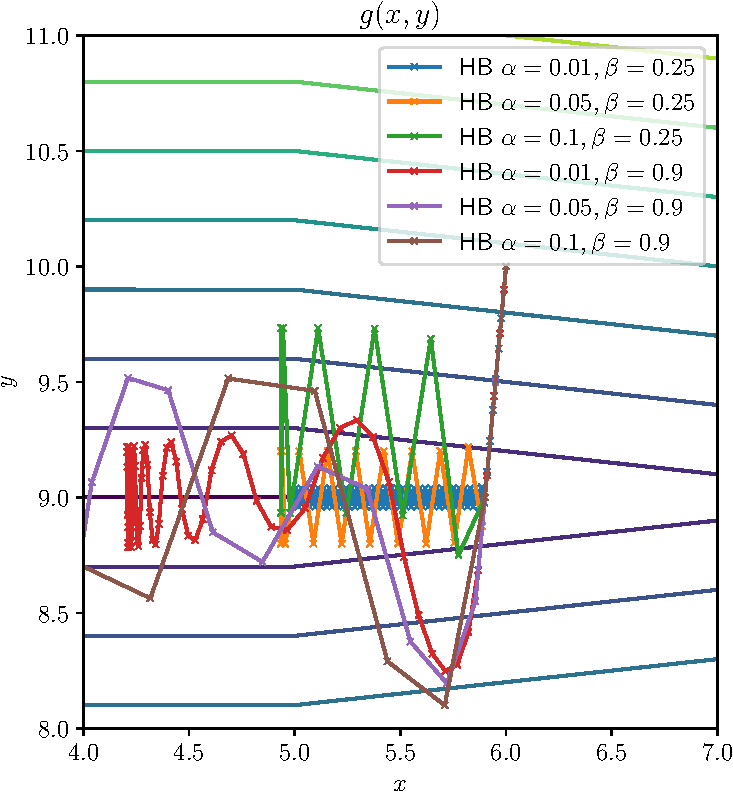
\includegraphics[width=0.45\textwidth]{fig/heavy_ball-step-plot-g.pdf}

    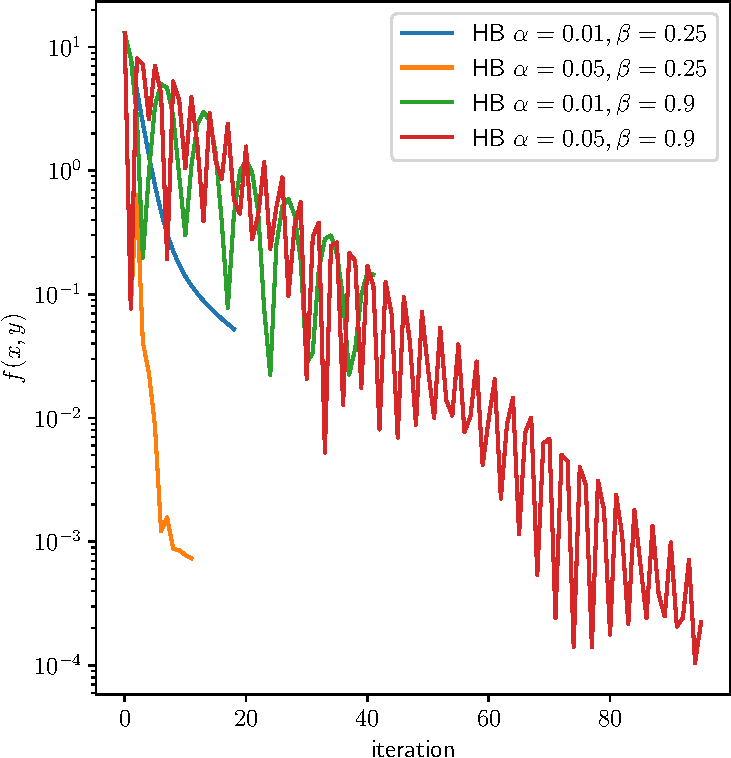
\includegraphics[width=0.45\textwidth]{fig/heavy_ball-iterations-f.pdf}
    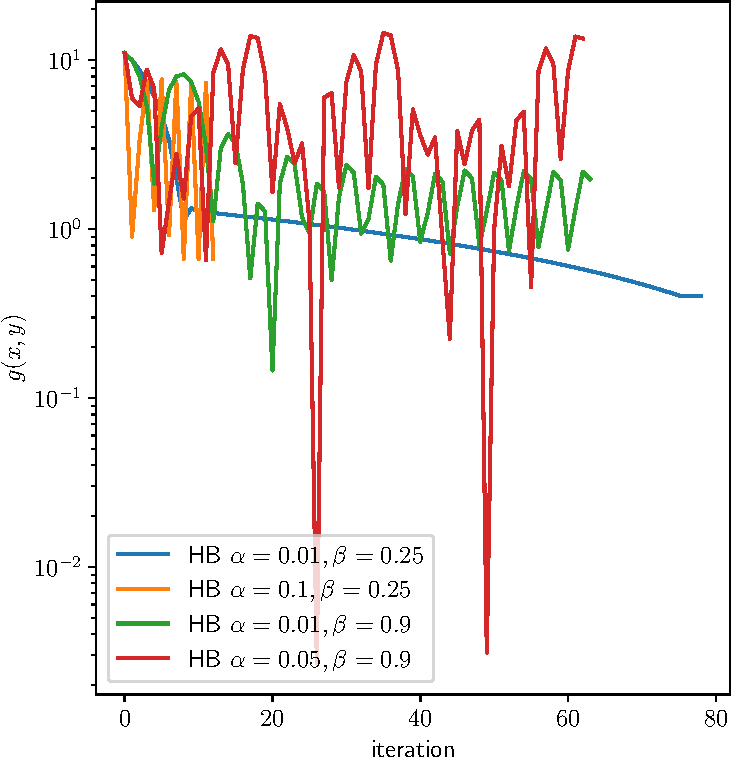
\includegraphics[width=0.45\textwidth]{fig/heavy_ball-iterations-g.pdf}
  \end{center}
  \caption{Various runs of gradient descent with different Heavy Ball hypers.}\label{fig:heavy_ball-step-plots}
\end{figure}


\subsection{(b) (iii) Adam hyperparameters}
Various runs of gradient descent with different Adam hyperparameters are presented
in Figure~\ref{fig:adam-step-plots}.
The $\beta_1$ parameter controls how quickly the momentum term decays, i.e.
how long the memory is for calculating momentum. The momentum for each
dimension $i$ is divided by another term $\epsilon + \sqrt{\hat v_i}$,
which is reminiscent of RMSProp. This term is also calculated in
terms of previous gradients, with length of memory controlled by $\beta_2$.

Of the parameters tested we find the best choice (while fixing $\alpha=0.01$) for
optimizing $f$ is $\beta_1=0.25$ and $\beta_2=0.25$. Increasing $\beta_1$ to 0.9
seems promising (initially optimizing faster than $\beta_1=0.25$),
but is cut off by our aggressive convergence condition.

For optimizing $g$ the choice of $\beta_1$ and $\beta_2$ has little impact.

Increasing $\alpha$ is generally beneficial, so long as it does not cause divergence,
and the choice of $\beta_1$ and $\beta_2$ influences how high we can push $\alpha$ without diverging.

\begin{figure}
  \begin{center}
    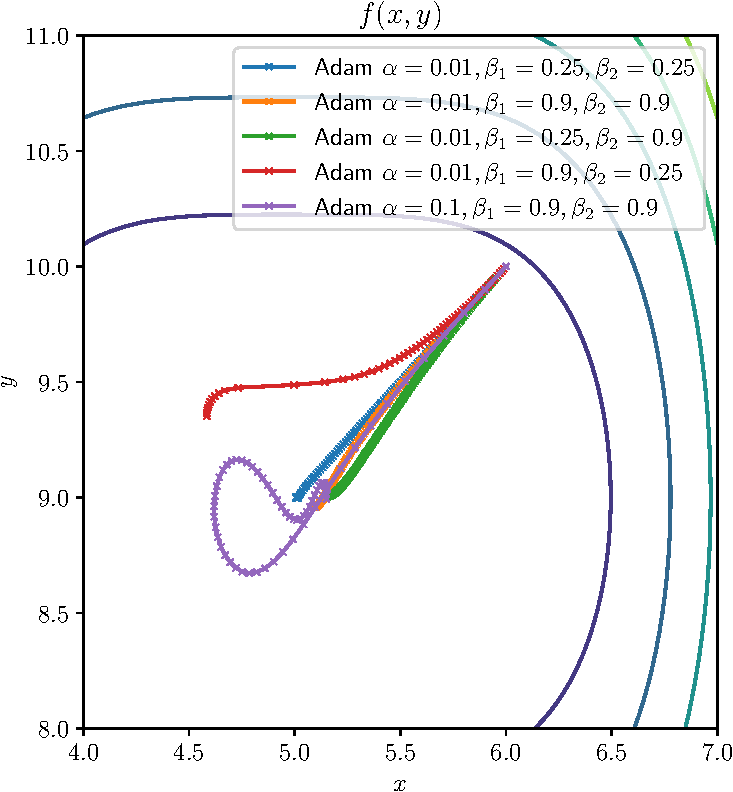
\includegraphics[width=0.45\textwidth]{fig/adam-step-plot-f.pdf}
    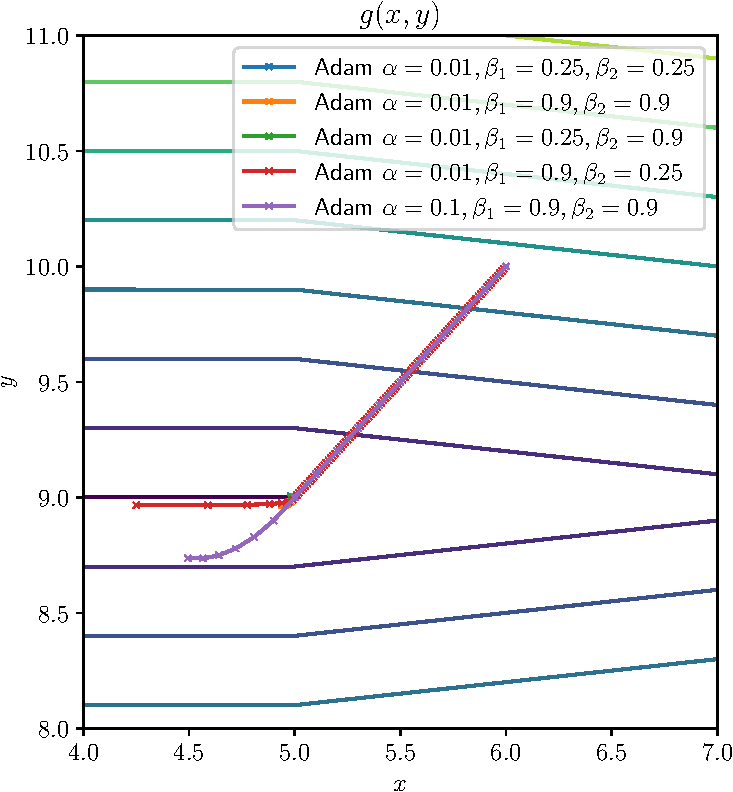
\includegraphics[width=0.45\textwidth]{fig/adam-step-plot-g.pdf}

    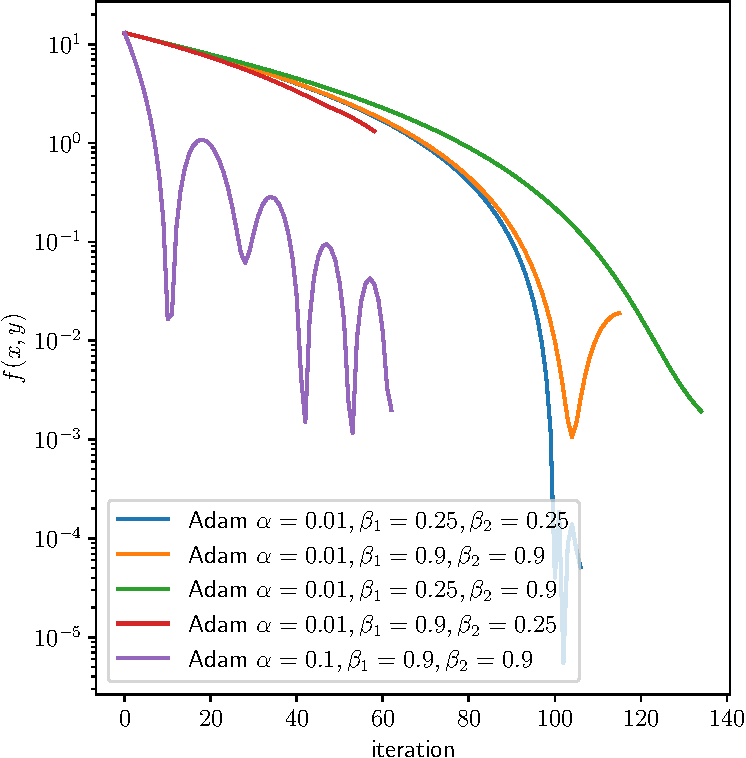
\includegraphics[width=0.45\textwidth]{fig/adam-iterations-f.pdf}
    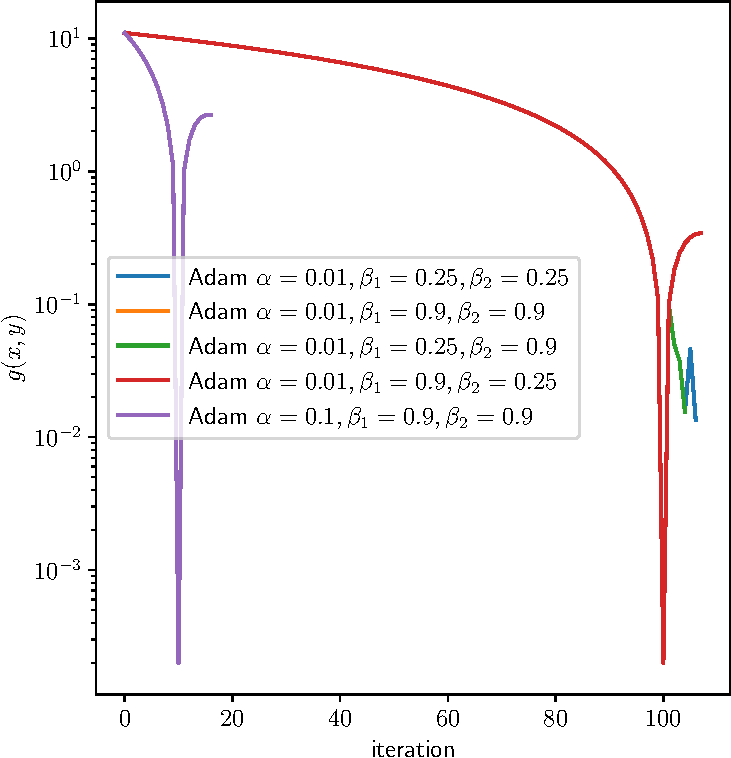
\includegraphics[width=0.45\textwidth]{fig/adam-iterations-g.pdf}
  \end{center}
  \caption{Various runs of gradient descent with different Adam hypers.}\label{fig:adam-step-plots}
\end{figure}

\section{(c)}
\subsection{(c) (i) ReLU with $x=-1$}
The derivative of the ReLU function is $0$ for all $x<0$.
Therefore all of the gradient descent step sizes, RMSProp, Adam, Heavy Ball,
result in the optimization procedure converging instantly, regardless of hyperparameters.
As it happens $x=-1$ also minimizes ReLU.

\subsection{(c) (ii) ReLU with $x=1$}
When we start at $x=1$ the gradient is non-zero so we actually have some movement.
For each of the algorithms the first step is small, and get's larger on successive iterations,
until the point where $x<0$. At this point the steps start to get smaller because each
of the algorithms more heavily discounts gradients further in the past.
Since each successive gradient after $x<0$ will be $0$ the step reduces until
the convergence condition is met.

In the case of RMSProp with $\beta=0.9$ and $\alpha=0.1$, the total number of iterations is 8,
but there is only one extra iteration after $x<0$.

For Heavy Ball with $\beta=0.9$ and $\alpha=0.1$, the function is minimized in only 5 iterations,
but it takes 63 iterations for the convergence condition to be met and for the algorithm to terminate.
The final estimate with this Heavy Ball configuration is $\approx-4$.
The ReLU function is acting like a ramp down which a ball rolls, giving it momentum to
glide some distance along the flat surface ($x<0$).

The Adam run with $\beta_1=0.9$ and $\beta_2=0.25$, $\alpha=0.1$, and $x_0=1$, starts off
with essentially constant step sizes, taking a step of $\approx0.1$ for the first 10 steps.
In this configuration it takes 139 iterations to reach the convergence condition, with
$x$ monotonically decreasing, and the final estimate being $-1746$.
The reason for this is that the $v$ term becomes very small amplifying the step size,
but because $\beta_1$ and $\beta_2$ are different, the $m$ term is not decreasing
as quickly.
Eventually $m$ becomes small enough to counteract the miniscule $v$.

\subsection{(c) (iii) ReLU with $x=100$}
In the case of RMSProp with $\beta=0.9$, $\alpha=0.1$, and $x_0=100$, the total number of iterations is 992,
and again there is only one extra iteration after $x<0$.
The final estimate is $-0.004$. The steps taken on each iteration are approximately constant at $0.1$.

For Heavy Ball with $\beta=0.9$, $\alpha=0.1$, and $x=100$, the function is minimized after only 109 iterations,
much faster than RMSProp with the same start.
However, it takes 175 iterations for the convergence condition to be met and for the algorithm to terminate.
The final estimate with this Heavy Ball configuration is $\approx-9$.
The step size starts out small at $0.1$ and increases to about $1$ by iteration 109, which
is the derivative of ReLU for $x>0$.

The Adam run with $\beta_1=0.9$ and $\beta_2=0.25$, $\alpha=0.1$, and $x_0=100$, 
takes 1000 iterations until $x<0$.
starts off with essentially constant step sizes, taking a step of $\approx0.1$ for the first 1000 steps.
In this configuration it takes 1133 iterations to reach the convergence condition, with
$x$ monotonically decreasing, and the final estimate being $-2431$.
The reason for this is that the $v$ term becomes very small amplifying the step size,
but because $\beta_1$ and $\beta_2$ are different, the $m$ term is not decreasing
as quickly.
Eventually $m$ becomes small enough to counteract the miniscule $v$.
The final value of $m$ is about $10^{-6}$, whereas the final value of $v$ is about  $10^{-80}$.
